\documentclass[sigconf]{acmart}

% ---- Clean workshop-draft top matter (relax for camera-ready) ----
\setcopyright{rightsretained}
\settopmatter{printacmref=false, printccs=false, printfolios=true}
\acmConference[MDE Intelligence '26]{8th Workshop on Artificial Intelligence and Model-Driven Engineering}{October 2026}{Malaga, Spain}
\acmYear{2026}
\acmISBN{}
\acmDOI{}
\renewcommand\footnotetextcopyrightpermission[1]{}

% ---- Packages (acmart already loads hyperref, xcolor, graphicx, amsmath) ----
\usepackage{booktabs}
\usepackage{array}
\usepackage{tabularx}
\usepackage{tikz}
\usetikzlibrary{positioning,shapes.geometric,arrows.meta,fit,backgrounds,calc}

% ---- TikZ styles ----
\tikzset{
  lang/.style={draw, rounded corners=2pt, fill=blue!8, font=\scriptsize, align=center, minimum height=6mm, inner sep=3pt},
  trans/.style={draw, ellipse, fill=black!6, font=\scriptsize, align=center, inner sep=2pt},
  act/.style={draw, rounded corners=3pt, font=\scriptsize, align=center, minimum height=7mm, minimum width=15mm, inner sep=2pt},
  obj/.style={draw, font=\scriptsize, align=center, fill=yellow!12, minimum height=6mm, inner sep=2pt},
  store/.style={draw, cylinder, shape border rotate=90, aspect=0.25, fill=green!8, font=\scriptsize, align=center, inner sep=2pt},
  ctrl/.style={draw, diamond, aspect=1.6, fill=orange!12, font=\scriptsize, align=center, inner sep=1pt},
  init/.style={draw, circle, fill=black, minimum size=3mm, inner sep=0pt},
  fin/.style={draw, circle, fill=black, minimum size=4mm, inner sep=0pt, label=center:{\color{white}\tiny$\blacksquare$}},
  cf/.style={-{Stealth[length=2mm]}, thick},
  df/.style={-{Stealth[length=2mm]}, dashed, gray}
}

\begin{document}

\title{Typing the Harness: Quality and Knowledge Debt in LLM-Assisted MDE}

% Single-blind venue: authored, not anonymized.
% Authors in alphabetical order by surname. TODO: confirm real emails (all placeholder)
% and Ha Phan's affiliation.
\author{Vasco Amaral}
\affiliation{%
  \institution{Universidade Nova de Lisboa}
  \city{Lisbon}
  \country{Portugal}}
\email{alfonso.pierantonio@univaq.it}
\author{Miguel Goul\~ao}
\affiliation{%
  \institution{Universidade Nova de Lisboa}
  \city{Lisbon}
  \country{Portugal}}
\email{alfonso.pierantonio@univaq.it}
\author{Ha Phan}
\affiliation{%
  \institution{Toronto Metropolitan University}
  \city{Toronto}
  \country{Canada}}
\email{alfonso.pierantonio@univaq.it}
\author{Alfonso Pierantonio}
\affiliation{%
  \institution{University of L'Aquila}
  \city{L'Aquila}
  \country{Italy}}
\email{alfonso.pierantonio@univaq.it}
\author{Manuel Wimmer}
\affiliation{%
  \institution{University of L'Aquila}
  \city{L'Aquila}
  \country{Italy}}
\email{alfonso.pierantonio@univaq.it}

\begin{abstract}
Large language model (LLM) agents now write a large share of the code in some model-driven engineering (MDE) tools, under human direction and across many sessions. The apparatus that makes this work, the harness, is a set of markup documents that carry intent, context, and verdicts between a human director and two agents, an architect and an implementer. These documents are the control surface of the process, yet their roles, the quality factors they serve, and how well an LLM actually exploits them are left informal. We abstract from a 320k-line MDE workbench, \texttt{Jjodel}, a reference harness: a triad of executors, a taxonomy of document types, a process model, and a phased evolution in which the process periodically rewrites itself through recalibration. We then characterize the harness in two complementary ways. A quality goal model (GRL/NFR) records what each document type is meant to improve, and what it harms, exposing three structural trade-offs. A performance characterization maps each document type to the typical characteristics of LLMs (context-window cost, long-context recall, instruction following, lazy loading, determinism). Knowledge debt is the gap between the two: where the intended quality contribution is not realized. We measure that gap on the \texttt{Jjodel} corpus of 346 documents and outline a cross-model validation with three LLMs (Claude, Gemini, Mistral) visualized as radar diagrams. The contribution is the reference harness, its quality and LLM-performance characterization, and knowledge debt cast as a measurable intended-versus-realized gap.
\end{abstract}

\keywords{model-driven engineering, large language models, harness engineering, goal modelling, quality attributes, knowledge debt, agentic development}

\maketitle

\section{Introduction}
A growing fraction of software, including MDE tooling, is now produced by LLM agents working under human direction. In the system we study the human author writes close to none of the code; the work is deciding what to build and maintaining the apparatus that lets agents build it reliably across sessions. That apparatus, the \emph{harness}, is a set of markup documents that carry intent, context, and verdicts between the agents. These documents are not passive notes: they are the control surface of the process.

The difficulty is that this control surface is informal. Documents accumulate, drift from the code, and encode assumptions that live only in the director's head. The accidental complexity of writing code has shrunk, but the essential complexity of keeping knowledge faithful to the system has not~\cite{brooks1987silverbullet}. We call the gap between the domain knowledge a document should incarnate and the knowledge actually internalized by its author or its consuming agents \emph{knowledge debt}, by analogy with technical debt~\cite{cunningham1992wycash,kruchten2012techdebt} but distinct from it: knowledge debt is about what the artifacts fail to carry, not about the quality of the code.

This paper abstracts a reusable harness from a real, heavily LLM-assisted MDE project and characterizes it along two axes. First, what each document type is \emph{meant} to achieve: which quality factors it improves and which it harms, captured as a goal model. Second, how each document type \emph{actually} fares given the characteristics of LLMs: context-window pressure, recall over long context, instruction following, lazy loading, determinism. Knowledge debt is the divergence between the two. We model the process structure as a plain flow of typed documents and steps, an activity-and-artifact process model, and keep that model deliberately lightweight.

\smallskip
\noindent\textbf{Research questions.}
\begin{description}
\item[RQ1] What process and document types constitute a reusable harness for LLM-assisted MDE development?
\item[RQ2] Which quality factors does each document type improve or harm, and what trade-offs result?
\item[RQ3] How does each document type perform with respect to LLM characteristics, and where does the intended quality contribution diverge from the realized one (knowledge debt)?
\end{description}

\noindent\textbf{Contributions.} (1) A reference harness abstracted from a 320k-line case: a triad of executors, a document taxonomy, a process model, and a phased evolution with recalibration as a self-referential meta-transformation. (2) A quality goal model of the harness, with a contribution matrix and three structural trade-offs. (3) A characterization of document-type performance against LLM characteristics. (4) Knowledge debt reframed as a measurable intended-versus-realized gap, quantified on \texttt{Jjodel} and with a cross-model validation design (Claude, Gemini, Mistral) visualized as radar diagrams.

\section{Background}
% TODO verify all footnote URLs and add access dates before submission.
LLM-based development has diversified into several styles that differ in how much autonomy the model is given, the unit of work it acts on, and the persistent artifacts it leaves behind. We review them in roughly increasing order of autonomy.

\emph{LLM chats} such as ChatGPT,\footnote{\url{https://chat.openai.com}} Gemini,\footnote{\url{https://gemini.google.com}} and Claude.ai\footnote{\url{https://claude.ai}} are general assistants: the developer describes a problem, the model returns code, and the developer pastes it back by hand. Nothing persists beyond the conversation, so the reasoning and the decisions live in an ephemeral session and are lost when it closes. This is where the project studied here began, cycling through several chat providers before settling on a structured loop.

\emph{LLM assistants} of the GitHub Copilot\footnote{\url{https://github.com/features/copilot}} kind move inside the editor, offering inline completion that the developer accepts or rejects at the level of tokens and lines. The underlying code models were popularized by Codex~\cite{chen2021codex}, and empirical work reports substantial productivity effects alongside usability and trust caveats~\cite{peng2023copilot,vaithilingam2022expectation}. The human stays in a tight review loop and little persists beyond the code itself.

\emph{LLM coding agents} such as Claude Code\footnote{\url{https://www.anthropic.com/claude-code}} and OpenAI Codex\footnote{\url{https://openai.com/codex}} take a whole task and edit the code base across many steps, reading the repository, running builds and tests, and iterating from a terminal. Autonomy rises from a single suggestion to a multi-step change, and with it the need to constrain the agent and to record what it did, typically through instruction files the agent reads before acting.

\emph{Intelligent IDEs} such as Cursor\footnote{\url{https://cursor.com}} and OpenCode\footnote{\url{https://opencode.ai}} embed these agents in the editor, adding repository-wide context, multi-file edits, and persistent project rules files that steer the agent across sessions.

\emph{Spec-driven development}, exemplified by Kiro\footnote{\url{https://kiro.dev}} and the broader spec-driven impulse~\cite{fowler2025specdriven}, inverts the flow: a structured specification (requirements, design, tasks) is authored first and drives generation, aiming at an auditable pipeline rather than ad hoc prompting.

Across these categories a common practice has emerged, largely independently: persistent instruction files that carry rules, conventions, and context to the model, from the constitution-like files coding agents read before each task to the rules and steering files of intelligent IDEs and spec-driven tools. This document layer is precisely what we call the harness. Yet a systematic review of LLMs for software engineering~\cite{hou2024llm4se} shows the literature concentrating on the model producing code; the documents that coordinate the process, and whether they preserve domain knowledge, receive little attention. Table~\ref{tab:aimodes} situates the categories. The harness studied here is a directed multi-agent setting in which a human director coordinates an architect and an implementer through a typed document set; our object of study is that document set, not the code generation itself.

\begin{table*}[t]
\caption{Categories of LLM-based development, by the human role, the unit of work, the persistent artifacts produced, and where the domain knowledge resides. The last row is the setting studied here.}
\label{tab:aimodes}
\small
\begin{tabularx}{\textwidth}{@{}p{3.6cm}p{2.5cm}p{2.1cm}XX@{}}
\toprule
Category (examples) & Human role & Unit of work & Persistent artifacts & Where knowledge lives \\
\midrule
LLM chat (ChatGPT, Gemini, Claude.ai) & prompter, copy-paste & snippet, file & ephemeral chat session & the session \\
LLM assistant, Copilot-like & reviewer of suggestions & token, line & none & model weights and code \\
LLM coding agent (Claude Code, Codex) & task-giver & task, feature & some (instructions, logs) & split between agent and code \\
Intelligent IDE (Cursor, OpenCode) & editor driver & multi-file edit & rules files, editor context & session and repository \\
Spec-driven development (Kiro) & specification author & spec to code & requirements, design, task docs & the specification \\
Directed multi-agent harness (this paper) & director who gates the loop & feature across roles & a typed document set & incarnated in the documents \\
\bottomrule
\end{tabularx}
\end{table*}

\section{Problems of LLM-based development}
Criticism of LLM-assisted development clusters around a few recognizable cores. We separate observable technical problems from the more structural epistemic and cognitive critiques, which are often the underestimated ones, and for each we note the lifecycle stage at which it surfaces (Table~\ref{tab:problems}).

\begin{table*}[t]
\caption{Typical problems of LLM-based development and the lifecycle stage at which each surfaces. Several originate at generation but only become visible later.}
\label{tab:problems}
\small
\begin{tabularx}{\textwidth}{@{}p{2.9cm}p{3.1cm}X@{}}
\toprule
Problem & Surfaces at (lifecycle stage) & Characterization \\
\midrule
Correctness and hallucination & generation; caught, if at all, at review and testing & Plausible but wrong code, invented APIs and library calls, no calibrated uncertainty; weak on concurrency, distributed systems, and non-local invariants that need global reasoning rather than pattern matching. \\
Security & generation; surfaces at build, testing, and in the supply chain & About 40\% of generated programs carry vulnerabilities~\cite{pearce2022asleep}; hallucinated package names enable slopsquatting~\cite{spracklen2025packages}; agentic flows add prompt injection. \\
Code quality and technical debt & originates at generation; paid at maintenance and evolution & More short-term churn, more copy-paste than refactoring, erosion of DRY and of architectural coherence~\cite{gitclear2024churn}. \\
Knowledge debt and cognitive atrophy & cross-cutting; design and maintenance; the team & One-shot artifacts skip the understanding normally built through construction; de-skilling and loss of the productive struggle that forms competence. Distinct from technical debt, and the focus of this paper. \\
Productivity, perception vs reality & whole lifecycle; verification overhead at review and testing & Experienced developers on their own repositories were 19\% slower with AI yet believed the opposite~\cite{metr2025productivity}; gains concentrate on boilerplate. \\
IP and provenance & generation; release; legal & Training on licensed code, verbatim regurgitation, opaque attribution and licensing.\footnote{See the {GitHub Copilot} litigation, \emph{Doe v.\ GitHub}, N.D.\ Cal., filed 2022; \url{https://githubcopilotlitigation.com}.} \\
Homogenization and regression to the mean & design and generation & Convergence on dominant corpus patterns, anchoring on the first suggestion, loss of solution diversity. \\
Evaluation and benchmarks & assessment, cross-cutting & Toy benchmarks such as HumanEval~\cite{chen2021codex}, test-set contamination, and weak correlation with real software engineering~\cite{hou2024llm4se}. \\
Context and scale limits & design and maintenance & No coherent global model of large systems, inconsistency from one session to the next. \\
\bottomrule
\end{tabularx}
\end{table*}

Two observations matter for the rest of the paper. First, the stage column shows that several problems are born at generation but become visible only later, at review, testing, or maintenance, which is exactly why a disciplined process with explicit review and recording steps can intercept them. Second, knowledge debt and cognitive atrophy stand apart: they are not defects in the code but in what the process fails to internalize, and unlike technical debt they escape any code-level check. This is the problem our harness is meant to expose and measure, and the one the rest of the paper operationalizes.

\section{A reference harness for LLM-assisted development}
We abstract the harness from \texttt{Jjodel}, a web-based MDE workbench (metamodelling, model editing, a transformation and an expression language, Ecore and XMI I/O) of about 320k lines, a large share produced by the implementer under direction.

\subsection{The triad}
The harness has three executors: a \emph{director} (human) who authors intent and gates the loop, an \emph{architect} (a conversational LLM) who reasons and generates prompts, and an \emph{implementer} (a coding agent) who edits the code base. The director plays two roles the model keeps apart: \emph{authoring} intent is an activity, while \emph{gating} (accept, reject, redirect) produces no artifact and is a decision. We record the executor of each step (director, architect, implementer, or collaborative) and whether the step is automatic (performed by an agent with no human action) or manual.

\subsection{Document taxonomy}
Table~\ref{tab:tax} lists the generic document types abstracted from the corpus, with their role and their primary writer and reader. The writer and reader are read off the process model (the executors of the steps that produce and consume a document type), not stored on the document.

\begin{table}[t]
\caption{Document taxonomy of the reference harness. Writer/reader are the executors of the producing/consuming steps. D director, A architect, I implementer.}
\label{tab:tax}
\scriptsize
\begin{tabularx}{\columnwidth}{@{}p{2.4cm}Xcc@{}}
\toprule
Document type & Role & W & R \\
\midrule
Persistent context & rules read before every task & A,D & A,I \\
Agent memory & distilled facts across sessions & A & A \\
Task brief & the director's intent & D & A \\
Design note & architect design and rationale & A & A,I \\
Discovery report & verdict on code-base state & A,I & D,A \\
Prompt artifact & instruction to the implementer & A & I \\
Specification & precise language or tool definition & A,D & A,I \\
Governance policy & conventions, standards, risk areas & D & A,I \\
Skill & lazily loaded competence & A,D & A,I \\
Operational log & append-only record & I & D,A \\
Handover or session & state passed between sessions & A & A \\
Code and changelog & the target and its record & I & A,I \\
Migration spec & realigns drifted artifacts & A & I \\
\bottomrule
\end{tabularx}
\end{table}

\subsection{The process}
Figure~\ref{fig:flow} shows the document-and-step structure and Figure~\ref{fig:proc} the enacted process. The running feature thread is: the director states intent, the architect produces a design and a discovery query, a discovery report comes back, the director gates on a risk and effort trade-off, the implementer changes the code, the change is committed, the log is appended. A step can consume and produce several document types (many-to-many), not just one.

\begin{figure}[t]
\centering
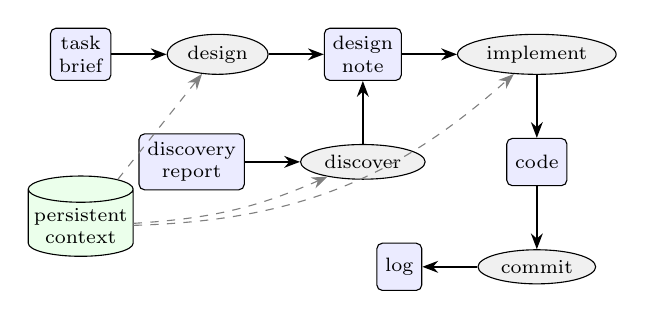
\begin{tikzpicture}[node distance=5mm and 7mm]
  \node[lang] (brief) {task\\brief};
  \node[trans, right=of brief] (tdes) {design};
  \node[lang, right=of tdes] (design) {design\\note};
  \node[trans, below=8mm of design] (tdisc) {discover};
  \node[lang, left=of tdisc] (disc) {discovery\\report};
  \node[trans, right=of design] (timpl) {implement};
  \node[lang, below=8mm of timpl] (code) {code};
  \node[trans, below=8mm of code] (tcom) {commit};
  \node[lang, left=of tcom] (log) {log};
  \node[store, below=12mm of brief] (claude) {persistent\\context};
  \draw[cf] (brief) -- (tdes);
  \draw[cf] (tdes) -- (design);
  \draw[cf] (disc) -- (tdisc);
  \draw[cf] (tdisc) -- (design);
  \draw[cf] (design) -- (timpl);
  \draw[cf] (timpl) -- (code);
  \draw[cf] (code) -- (tcom);
  \draw[cf] (tcom) -- (log);
  \draw[df] (claude) -- (tdes);
  \draw[df] (claude) to[bend right=10] (tdisc);
  \draw[df] (claude) to[bend right=20] (timpl);
\end{tikzpicture}
\caption{Document types (boxes) and the steps (ovals) that produce and consume them. Persistent context (cylinder) is read by many steps. The full harness has 11 document types and 13 steps.}
\label{fig:flow}
\end{figure}

\begin{figure}[t]
\centering
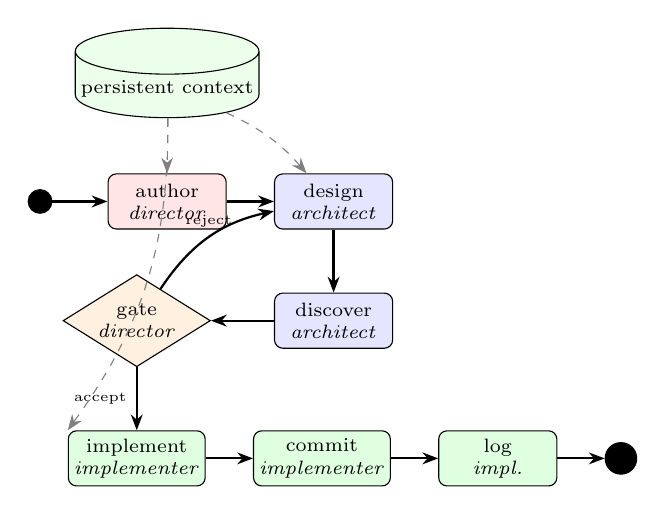
\begin{tikzpicture}[node distance=4mm and 6mm]
  \node[init] (i) {};
  \node[act, right=7mm of i, fill=red!10] (author) {author\\\textit{director}};
  \node[act, right=of author, fill=blue!10] (design) {design\\\textit{architect}};
  \node[act, below=8mm of design, fill=blue!10] (discover) {discover\\\textit{architect}};
  \node[ctrl, left=8mm of discover] (gate) {gate\\\textit{director}};
  \node[act, below=8mm of gate, fill=green!12] (impl) {implement\\\textit{implementer}};
  \node[act, right=of impl, fill=green!12] (commit) {commit\\\textit{implementer}};
  \node[act, right=of commit, fill=green!12] (logA) {log\\\textit{impl.}};
  \node[fin, right=6mm of logA] (f) {};
  \node[store, above=7mm of author] (cl) {persistent context};
  \draw[cf] (i) -- (author);
  \draw[cf] (author) -- (design);
  \draw[cf] (design) -- (discover);
  \draw[cf] (discover) -- (gate);
  \draw[cf] (gate) -- node[font=\tiny,left]{accept} (impl);
  \draw[cf] (gate) to[bend left=22] node[font=\tiny,above]{reject} (design);
  \draw[cf] (impl) -- (commit);
  \draw[cf] (commit) -- (logA);
  \draw[cf] (logA) -- (f);
  \draw[df] (cl) -- (author);
  \draw[df] (cl) to[bend left=12] (design);
  \draw[df] (cl) to[bend left=18] (impl.north west);
\end{tikzpicture}
\caption{The enacted process. Activities are coloured by executor; the gate is a decision with a reject back-edge; persistent context feeds several activities by data flow (dashed).}
\label{fig:proc}
\end{figure}

\subsection{Evolution and recalibration}
The harness is not static. It evolved through four phases of LLM adoption (Figure~\ref{fig:phases}): a spontaneous phase with a single chat and no documents; a three-agent phase introducing a persistent constitution; an intermediate phase adding handover documents for design coherence; and the current phase of code-base support documents (discovery reports, session and prompt documents, decision and operational logs). Transitions are not drift but \emph{recalibration} events in which the architect and implementer analyse the code base and the director gates a change to the process itself. Recalibration is therefore a self-referential meta-transformation,
\(\textsf{Recalibrate}: (\textit{CodeBase}, \textit{Harness}_n) \rightarrow \textit{Harness}_{n+1}\),
whose output is a new set of document types and steps for the process that runs it. The model in this paper is the current-phase snapshot; earlier document types such as handover carry a validity interval.

\begin{figure}[t]
\centering
\resizebox{\columnwidth}{!}{% Harness evolution timeline: four phases with recalibration meta-transformations.
% Embeddable via \input; needs tikz with positioning, arrows.meta, shapes.geometric (loaded in main.tex).
% Namespaced styles (ph, rec, rarr) avoid clashes.
\tikzset{
  ph/.style={draw, rounded corners=2pt, align=center, font=\tiny, inner sep=3pt, minimum height=15mm, fill=blue!7, text width=20mm},
  rec/.style={draw, circle, fill=orange!18, font=\tiny\bfseries, inner sep=1pt, minimum size=6mm},
  flow/.style={-{Stealth[length=2mm]}, thick},
  selfp/.style={-{Stealth[length=1.6mm]}, orange!70!black}
}
\begin{tikzpicture}[x=1mm, y=1mm]
  \node[ph, fill=black!4] (p1) at (0,0)   {\textbf{1. Spontaneous}\\\textit{pre-2026-01}\\human + 1 chat\\(GPT, Gemini, Claude)\\\textbf{docs: none}};
  \node[ph] (p2) at (30,0)  {\textbf{2. Three agents}\\\textit{2026-01-17}\\director, architect,\\implementer\\\textbf{constitution}};
  \node[ph] (p3) at (60,0)  {\textbf{3. Intermediate+}\\\textit{2026-01-22 to 02}\\same triad\\\textbf{handover docs}};
  \node[ph, fill=green!8] (p4) at (90,0) {\textbf{4. Codebase docs}\\\textit{2026-03 to 06}\\same triad\\\textbf{discovery, session,}\\\textbf{prompt, logs}};

  \node[rec] (r1) at (15,0) {R};
  \node[rec] (r2) at (45,0) {R};
  \node[rec] (r3) at (75,0) {R};

  \draw[flow] (p1) -- (r1); \draw[flow] (r1) -- (p2);
  \draw[flow] (p2) -- (r2); \draw[flow] (r2) -- (p3);
  \draw[flow] (p3) -- (r3); \draw[flow] (r3) -- (p4);

  % self-reference: recalibration reads the codebase and rewrites the harness
  \draw[selfp] (r2) to[out=110,in=70,looseness=6] (r2);
  \node[font=\tiny, orange!60!black] at (45,11) {self-rewrite};

  \node[font=\tiny, align=center] at (45,-13)
    {\textbf{R} = recalibration: architect + implementer analyse the codebase, director gates the change to the harness};
\end{tikzpicture}
}
\caption{Harness evolution: four phases of LLM adoption with recalibration (R) as a self-referential meta-transformation. Dates are anchored to git history.}
\label{fig:phases}
\end{figure}

\section{A quality goal model of the harness}
The goal model (Figure~\ref{fig:goal}) records, for each document type, the quality factors it is designed to improve or harm. Following the NFR framework and GRL, quality factors are softgoals and document types are operationalizations contributing positively or negatively to them. Two top softgoals are in tension, knowledge fidelity (consistency, freshness, traceability, coverage, reproducibility, comprehensibility) and process efficiency (token economy, velocity), with governance (conformance, risk containment) cross-cutting. Table~\ref{tab:matrix} is the full contribution matrix.

\begin{figure}[t]
\centering
\resizebox{\columnwidth}{!}{% Softgoal interdependency graph (NFR / GRL) for the harness.
% Embeddable via \input; requires tikz with libraries positioning, shapes.geometric, arrows.meta
% (all already loaded in main.tex). Styles are namespaced (sg, sgtop, op, pos, neg, dec) to avoid
% clashing with the FTG/PM styles in main.tex.
\tikzset{
  sg/.style={draw, ellipse, fill=blue!6, font=\tiny, align=center, inner sep=1.4pt, minimum width=13mm},
  sgtop/.style={draw, ellipse, fill=blue!14, font=\scriptsize, align=center, inner sep=2pt, thick, minimum width=20mm},
  op/.style={draw, rounded corners=2pt, fill=yellow!14, font=\tiny, align=center, inner sep=2pt, minimum height=5.5mm},
  hlp/.style={-{Stealth[length=1.6mm]}, green!55!black, semithick},
  hrt/.style={-{Stealth[length=1.6mm]}, red!75!black, dashed, semithick},
  dec/.style={-{Stealth[length=1.4mm]}, black!45},
  lbl/.style={fill=white, inner sep=0.5pt, font=\tiny}
}
\begin{tikzpicture}[x=1mm, y=1mm]
  % --- leaf softgoals (quality factors) ---
  \node[sg] (cons)  at (0,0)    {Consistency};
  \node[sg] (fresh) at (23,0)   {Freshness};
  \node[sg] (trac)  at (46,0)   {Traceability};
  \node[sg] (repr)  at (69,0)   {Reproducib.};
  \node[sg] (tok)   at (92,0)   {Token\\economy};
  \node[sg] (risk)  at (115,0)  {Risk\\containment};

  % --- top softgoals ---
  \node[sgtop] (kf) at (34,22) {Knowledge\\fidelity};
  \node[sgtop] (pe) at (92,22) {Process\\efficiency};
  \node[sgtop] (gov) at (115,22) {Governance};

  % --- decomposition links (leaf -> top) ---
  \draw[dec] (cons)  -- (kf);
  \draw[dec] (fresh) -- (kf);
  \draw[dec] (trac)  -- (kf);
  \draw[dec] (repr)  -- (kf);
  \draw[dec] (tok)   -- (pe);
  \draw[dec] (risk)  -- (gov);

  % --- operationalizations (document types) ---
  \node[op] (pc)   at (8,-24)   {Persistent\\context};
  \node[op] (spec) at (40,-24)  {Specification};
  \node[op] (skill)at (80,-24)  {Skill};
  \node[op] (disc) at (112,-24) {Discovery\\report};

  % --- contribution links ---
  % Persistent context: trade-off 1 (fidelity vs token) + freshness liability
  \draw[hlp] (pc) -- (cons.south)  node[lbl,pos=0.35]{++};
  \draw[hrt] (pc) to[bend right=14] (tok) node[lbl,pos=0.62]{$--$};
  \draw[hrt] (pc) -- (fresh) node[lbl,pos=0.6]{$-$};
  % Specification: trade-off 2 (consistency vs freshness)
  \draw[hlp] (spec) -- (cons.south east) node[lbl,pos=0.55]{++};
  \draw[hrt] (spec) -- (fresh) node[lbl,midway]{$-$};
  % Skill: trade-off 3 (efficiency vs determinism/risk)
  \draw[hlp] (skill) -- (tok) node[lbl,midway]{++};
  \draw[hlp] (skill) -- (repr) node[lbl,pos=0.55]{$+$};
  \draw[hrt] (skill) -- (risk) node[lbl,pos=0.6]{$-$};
  % Discovery report: intended traceability vs realized (the debt gap) + risk containment
  \draw[hlp] (disc) -- (risk) node[lbl,midway]{++};
  \draw[hlp] (disc) to[bend right=10] (trac) node[lbl,pos=0.5]{$+$};
  \draw[hrt] (disc) to[bend left=22] node[lbl,pos=0.5]{realized $\approx 0$} (trac);

  % --- tension between the two top softgoals ---
  \draw[{Stealth[length=1.6mm]}-{Stealth[length=1.6mm]}, red!75!black, thick] (kf) -- node[lbl]{conflict} (pe);

  % --- legend ---
  \node[font=\tiny, anchor=west, align=left] at (-2,-40)
    {\textcolor{green!55!black}{$\rightarrow$} Help/Make ($+,++$)\quad
     \textcolor{red!75!black}{$\rightarrow$} Hurt/Break ($-,--$, dashed)\quad
     \textcolor{black!45}{$\rightarrow$} decomposition};
\end{tikzpicture}
}
\caption{Softgoal interdependency graph of the harness. Document types (operationalizations) contribute Help/Make or Hurt/Break to quality factors. The three structural trade-offs and the discovery report's intended-versus-realized traceability gap are highlighted.}
\label{fig:goal}
\end{figure}

\begin{table*}[t]
\caption{Contribution matrix: how each document type affects each quality factor. ++ Make, + Help, $-$ Hurt, $--$ Break. Cons consistency, Fresh freshness, Trac traceability, Cov coverage, Repr reproducibility, Comp comprehensibility, Tok token economy, Vel velocity, Conf conformance, Risk risk containment.}
\label{tab:matrix}
\small
\begin{tabular}{@{}lcccccccccc@{}}
\toprule
Document type & Cons & Fresh & Trac & Cov & Repr & Comp & Tok & Vel & Conf & Risk \\
\midrule
Persistent context & ++ & $-$ & & + & + & + & $--$ & & + & + \\
Agent memory & + & $-$ & + & & & + & $-$ & + & & \\
Task brief & + & & + & + & & + & & + & & \\
Design note & + & & + & + & & ++ & $-$ & & & \\
Discovery report & + & & + & + & & + & + & + & & ++ \\
Prompt artifact & + & & + & & + & + & & + & + & + \\
Specification & ++ & $-$ & & + & + & ++ & $-$ & & + & \\
Governance policy & + & & & + & + & + & $--$ & & ++ & + \\
Skill & + & & & + & + & + & ++ & + & + & $-$ \\
Operational log & & & ++ & + & & & $--$ & & + & \\
Handover or session & + & $-$ & + & & & + & $-$ & + & & \\
Code and changelog & & & + & ++ & & & & & & + \\
Migration spec & ++ & + & & & + & & & & + & + \\
\bottomrule
\end{tabular}
\end{table*}

The matrix exposes three structural trade-offs. First, token economy versus knowledge fidelity: nearly every fidelity-improving document hurts token economy by competing for the context window or loading every session; the skill resolves this by loading lazily. Second, freshness versus consistency: persistent stores Make consistency but are themselves freshness liabilities as the code moves. Third, determinism versus efficiency: the skill Helps reproducibility yet Hurts risk containment because its selection is non-deterministic.

\section{Document performance under LLM characteristics}
The goal model is design intent. Whether a document realizes that intent depends on how an LLM consumes it. We characterize each document type against five LLM characteristics: context-window cost (how much it occupies), long-context recall (lost-in-the-middle exposure), instruction-following load, lazy-loadability, and determinism of use. Table~\ref{tab:llm} summarizes the salient interactions.

\begin{table}[t]
\caption{Document performance under LLM characteristics. CW context-window cost, RC long-context recall risk, IF instruction-following load, LL lazy-loadable, DET determinism of use. H high, M medium, L low.}
\label{tab:llm}
\scriptsize
\begin{tabularx}{\columnwidth}{@{}Xccccc@{}}
\toprule
Document type & CW & RC & IF & LL & DET \\
\midrule
Persistent context & H & H & H & no & H \\
Governance policy & H & M & H & part & H \\
Specification & H & H & M & part & H \\
Discovery report & M & M & L & yes & M \\
Skill & L & L & M & yes & L \\
Operational log & H & L & L & yes & H \\
\bottomrule
\end{tabularx}
\end{table}

The characterization explains the trade-offs mechanically. The persistent context maximizes consistency but its high context-window cost and recall risk mean that as it grows, the probability that a given rule is actually attended to falls (lost-in-the-middle). The skill is the harness's response: it converts a high context-window cost into an on-demand load, at the price of a non-deterministic selection step. The operational log is cheap to consult on demand but expensive if kept unbounded in context, which is exactly where its stated rotation rule matters.

\section{Knowledge debt as the intended-versus-realized gap}
Knowledge debt is where a document's realized contribution falls short of its intended one. The goal model gives the intended contribution; an audit of the corpus gives the realized one; each negative realized link overriding a positive intended link is a debt instance. In process terms the gap surfaces as a conformance failure of the enacted process against its intended document-and-step model, of six kinds: a document that no type covers (missing document type); a real step that no defined step covers (missing step); a persistent store whose content no longer matches the code (stale context); a step whose output never appears as a written document (dead step); an activity reading a long-stale document (stale read); and a transient handoff carrying assumptions absent from every document type's definition (undocumented knowledge in transit).

We measured these on the \texttt{Jjodel} corpus of 346 authored documents at a fixed commit; every figure is scripted and re-runnable (Table~\ref{tab:ind}). Two results are sharp. \textbf{Handoff incarnation.} Of 193 discovery reports, excluding the append-only log, only 7 (about 3.6 percent) are referenced by any downstream design, spec, or implementation document. The discovery report's intended traceability contribution is therefore realized only marginally: the knowledge stays in session. \textbf{Governance conformance.} The persistent context states a rotation invariant for the log (keep the last 20 entries, archive the rest); the active log holds 657 entries and no archive exists, a violation by a factor of about 33. The document asserts a rule the process does not keep.

\begin{table}[t]
\caption{Measured indicators on \texttt{Jjodel} at a fixed commit. All static (computable from model and corpus).}
\label{tab:ind}
\small
\begin{tabularx}{\columnwidth}{@{}Xl@{}}
\toprule
Indicator & Value \\
\midrule
Document typing coverage & $\approx$67\% (233/346) \\
Handoff incarnation rate & $\approx$3.6\% (7/193) \\
Persistent-context freshness & both stores now maintained \\
Governance-rule conformance & 1 invariant violated 33$\times$ \\
Retired-step fraction & 1 of 13 document types \\
Derived-doc drift & 3--4\% size of source spec \\
Type-authority presence & absent (metamodel file) \\
\bottomrule
\end{tabularx}
\end{table}

\section{Validation across models}
The indicators above are static, computed on documents. A complementary question is whether document-type performance (Section~6) holds across LLMs. We outline a controlled protocol and visualize it as radar diagrams; data collection is ongoing and the values in Figure~\ref{fig:radar} are illustrative placeholders.

\paragraph{Protocol.} For each document type, the same controlled task is given to three models, Claude, Gemini, and Mistral, on five measurable axes: instruction adherence (does the model follow the document), factual recall (does it retrieve facts the document states), output conformance (does its output obey the document), token efficiency (cost to achieve the above), and position robustness (does adherence survive when the document is placed late in a long context). Each axis is scored on a normalized scale by an objective check where possible. Three models is illustrative, not a definitive comparison.

\begin{figure}[t]
\centering
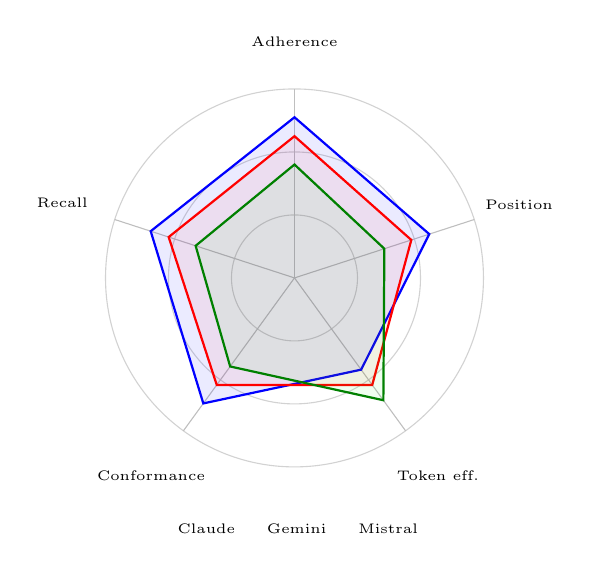
\begin{tikzpicture}
  \def\R{24mm}
  \foreach \r in {8mm,16mm,24mm} \draw[gray!35] (0,0) circle (\r);
  \foreach \ang in {90,162,234,306,18} \draw[gray!50] (0,0) -- (\ang:\R);
  \node[font=\tiny] at (90:30mm) {Adherence};
  \node[font=\tiny] at (162:31mm) {Recall};
  \node[font=\tiny] at (234:31mm) {Conformance};
  \node[font=\tiny] at (306:31mm) {Token eff.};
  \node[font=\tiny] at (18:30mm) {Position};
  % Claude (illustrative)
  \draw[blue,thick,fill=blue,fill opacity=0.08]
    (90:20.4mm) -- (162:19.2mm) -- (234:19.7mm) -- (306:14.4mm) -- (18:18mm) -- cycle;
  % Gemini (illustrative)
  \draw[red,thick,fill=red,fill opacity=0.06]
    (90:18mm) -- (162:16.8mm) -- (234:16.8mm) -- (306:16.8mm) -- (18:15.6mm) -- cycle;
  % Mistral (illustrative)
  \draw[green!50!black,thick,fill=green,fill opacity=0.06]
    (90:14.4mm) -- (162:13.2mm) -- (234:13.9mm) -- (306:19.2mm) -- (18:12mm) -- cycle;
  \node[font=\tiny, anchor=north] at (0,-30mm)
    {\textcolor{blue}{$\blacksquare$} Claude \quad \textcolor{red}{$\blacksquare$} Gemini \quad \textcolor{green!50!black}{$\blacksquare$} Mistral};
\end{tikzpicture}
\caption{Illustrative radar of document-type performance across three models on the five protocol axes. Values are placeholders pending the measured run.}
\label{fig:radar}
\end{figure}

\section{Discussion and threats to validity}
The study is n equals 1: one harness and one director, who is also the analyst, assisted by the same family of agents that run the harness. Generality is not claimed; the contribution is a reusable harness and a characterization method. Several indicators depend on classification choices a reviewer can contest (what counts as a downstream consumer, as cleanly typed); we report the rules so they can be reproduced. The goal-model contributions are first-pass and partly judgement-based; each strong link should be justified against evidence or revised. The cross-model validation is designed but not yet run, and three models are illustrative. The mechanism of skill selection is treated as inference over concepts rather than lexical match, supported by interpretability evidence~\cite{templeton2024monosemanticity}; the opposing probabilistic reading is also tenable and we do not adjudicate it.

\section{Related work}
\textbf{AI in software development.} Work ranges from inline completion and its productivity studies~\cite{chen2021codex,peng2023copilot,vaithilingam2022expectation} to agentic coding, surveyed broadly in~\cite{hou2024llm4se}; the focus is the model producing code. We instead model the process and the documents that coordinate it. \textbf{Goal and quality modelling.} The NFR framework and GRL model softgoals and their contributions; we apply them to development-process documents rather than to a system under design. \textbf{Process modelling.} Strict workflows gave way to declarative process models~\cite{pesic2006declare} and to conformance checking and process mining over logs~\cite{vanderaalst2016processmining}; our process is director-driven yet internally non-deterministic, which points to property checking over traces. \textbf{Technical versus knowledge debt.} Technical debt is a property of the code~\cite{cunningham1992wycash,kruchten2012techdebt}; knowledge debt, as we use it, is a property of the documents and their conformance to a model of the process.

\section{Conclusion and future work}
We abstracted a reusable harness for LLM-assisted MDE development (RQ1), characterized each document type by the quality factors it serves and harms, with three trade-offs (RQ2), and mapped document types to LLM characteristics, defining knowledge debt as the intended-versus-realized gap and measuring it on a real corpus (RQ3). The reference harness, the quality and LLM-performance characterization, and the gap framing are the contribution. Future work completes the cross-model radar study, plots debt across phases rather than at one instant, and feeds the validated model back into a recalibration to generate the next harness.

\bibliographystyle{ACM-Reference-Format}
\bibliography{references}

\end{document}
